\documentclass[12pt,letterpaper]{article}
\usepackage[utf8]{inputenc}
\usepackage[margin=.5in]{geometry}
\usepackage{graphicx}
\usepackage{titling}
\usepackage{amsmath}
\usepackage{amsfonts}
\usepackage{amssymb}
\renewcommand{\theenumiv}{\arabic{enumiv}}
\setlength{\droptitle}{-5em}
\author{Maurice Diesendruck}
\title{StatMod2 - Backfitting - Exercises 4}
\usepackage{Sweave}
\begin{document}
\input{statmod-backfitting-concordance}
\maketitle


\section{Model}

Constraining $\hat{\alpha}$ to be the sample average of $y$, 
removes issues of unidentifiability.\\

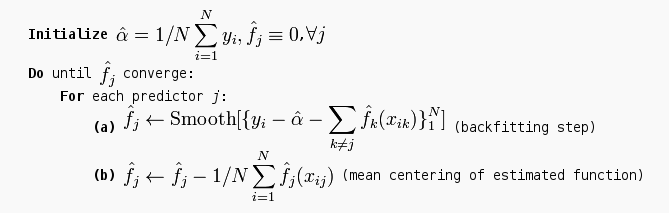
\includegraphics[width=.7\textwidth]{backfitting-function.png}

\section{Results}

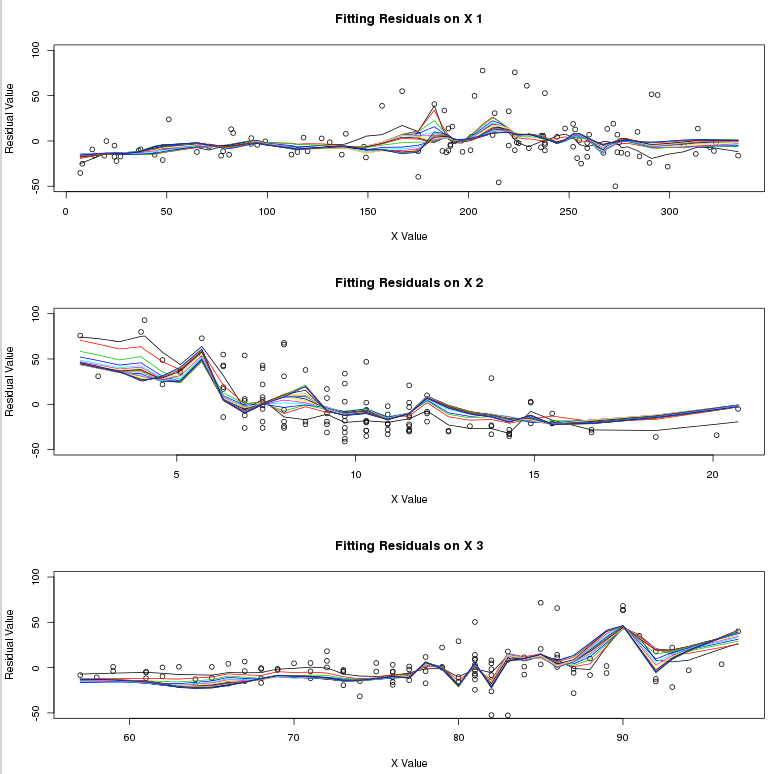
\includegraphics[width=.7\textwidth]{backfitting.png}

\begin{Schunk}
\begin{Sinput}
> # StatMod2 - Backfitting HW - Exercices 4
> 
> library(stats)
> #setwd("~/Google Drive/2. SPRING 2015/STAT MOD 2 - Prof Scott/backfitting")
> setwd("~/Documents/latex")
> data <- read.csv("air.csv")
> data <- data[order(data[, 1]), ]
> y <- as.matrix(data$Ozone)
> x <- data[,c("Solar.R","Wind","Temp")]
> n <- length(data[,1])
> p <- dim(x)[2]
> times <- 20
> # Initialize alpha, f, and mses.
> a <- mean(y)
> f <- array(0, dim=c(p, n))
> mses <- NULL
> Backfit <- function(q) {
+   
+   # Do t iterations.
+   for (t in 1:times) {
+     # Rather than convergence, I record all MSEs for review, below.
+     
+     # Do for each partial residual (kth predictor).
+     #for (k in c(1, 2, 3)) {
+     #for (k in c(3, 2, 1)) {
+     for (k in c(2, 1, 3)) {
+       
+       # Remove one column, to make p-1 by 1 matrix.
+       f.minus.k <- as.matrix(f[-k,])
+       
+       # Prepare value to smooth; the Yi - a - sum(...).
+       to.smooth <- rep(0, n)
+       for (i in 1:n) {
+         to.smooth[i] <- y[i] - a - sum(f.minus.k[,i])
+       }
+       
+       # Fit kth residual against kth column of x.
+       partial.data <- cbind(y, x[k],to.smooth)
+       partial.data <- partial.data[order(partial.data[,2]),]
+       predicted <- rep(0, n)
+       predicted <- lowess(partial.data[,c(2,3)], f=.1)$y
+      
+       # Plot stuff.
+       if (k==q) {
+         if (t==1) {
+           plot(t(x[k]), to.smooth, main=paste("Fitting Residuals on X", k),
+                ylim=c(-50,100), xlab="X Value", ylab="Residual Value")
+         }
+         lines(partial.data[,2], predicted, col=t)
+       }
+       
+       # Attach predicted values to a resorted (by y) matrix.
+       to.sort <- cbind(partial.data, predicted)
+       resorted <- to.sort[order(to.sort[,1]),]
+       # Record K-th predictor for t-th iteration.
+       f[k,] <- resorted$predicted - mean(resorted$predicted)
+     }
+   
+     mses[t] <- (1/n)*sum((y - a - colSums(f))^2)
+   }
+   return (mses)
+ }
> par(mfrow=c(3,1))
> for (q in 1:p) {
+   mses <- Backfit(q)
+ }
> summary(mses)
\end{Sinput}
\begin{Soutput}
   Min. 1st Qu.  Median    Mean 3rd Qu.    Max. 
  207.9   210.9   229.0   240.1   257.6   366.0 
\end{Soutput}
\end{Schunk}

\end{document}
